\documentclass[9pt,a4paper,]{extarticle}

\usepackage{f1000_styles}

\usepackage[pdfborder={0 0 0}]{hyperref}

\usepackage[numbers]{natbib}


%% maxwidth is the original width if it is less than linewidth
%% otherwise use linewidth (to make sure the graphics do not exceed the margin)
\makeatletter
\def\maxwidth{ %
  \ifdim\Gin@nat@width>\linewidth
    \linewidth
  \else
    \Gin@nat@width
  \fi
}
\makeatother

\usepackage{color}
\usepackage{fancyvrb}
\newcommand{\VerbBar}{|}
\newcommand{\VERB}{\Verb[commandchars=\\\{\}]}
\DefineVerbatimEnvironment{Highlighting}{Verbatim}{commandchars=\\\{\}}
% Add ',fontsize=\small' for more characters per line
\usepackage{framed}
\definecolor{shadecolor}{RGB}{248,248,248}
\newenvironment{Shaded}{\begin{snugshade}}{\end{snugshade}}
\newcommand{\KeywordTok}[1]{\textcolor[rgb]{0.13,0.29,0.53}{\textbf{#1}}}
\newcommand{\DataTypeTok}[1]{\textcolor[rgb]{0.13,0.29,0.53}{#1}}
\newcommand{\DecValTok}[1]{\textcolor[rgb]{0.00,0.00,0.81}{#1}}
\newcommand{\BaseNTok}[1]{\textcolor[rgb]{0.00,0.00,0.81}{#1}}
\newcommand{\FloatTok}[1]{\textcolor[rgb]{0.00,0.00,0.81}{#1}}
\newcommand{\ConstantTok}[1]{\textcolor[rgb]{0.00,0.00,0.00}{#1}}
\newcommand{\CharTok}[1]{\textcolor[rgb]{0.31,0.60,0.02}{#1}}
\newcommand{\SpecialCharTok}[1]{\textcolor[rgb]{0.00,0.00,0.00}{#1}}
\newcommand{\StringTok}[1]{\textcolor[rgb]{0.31,0.60,0.02}{#1}}
\newcommand{\VerbatimStringTok}[1]{\textcolor[rgb]{0.31,0.60,0.02}{#1}}
\newcommand{\SpecialStringTok}[1]{\textcolor[rgb]{0.31,0.60,0.02}{#1}}
\newcommand{\ImportTok}[1]{#1}
\newcommand{\CommentTok}[1]{\textcolor[rgb]{0.56,0.35,0.01}{\textit{#1}}}
\newcommand{\DocumentationTok}[1]{\textcolor[rgb]{0.56,0.35,0.01}{\textbf{\textit{#1}}}}
\newcommand{\AnnotationTok}[1]{\textcolor[rgb]{0.56,0.35,0.01}{\textbf{\textit{#1}}}}
\newcommand{\CommentVarTok}[1]{\textcolor[rgb]{0.56,0.35,0.01}{\textbf{\textit{#1}}}}
\newcommand{\OtherTok}[1]{\textcolor[rgb]{0.56,0.35,0.01}{#1}}
\newcommand{\FunctionTok}[1]{\textcolor[rgb]{0.00,0.00,0.00}{#1}}
\newcommand{\VariableTok}[1]{\textcolor[rgb]{0.00,0.00,0.00}{#1}}
\newcommand{\ControlFlowTok}[1]{\textcolor[rgb]{0.13,0.29,0.53}{\textbf{#1}}}
\newcommand{\OperatorTok}[1]{\textcolor[rgb]{0.81,0.36,0.00}{\textbf{#1}}}
\newcommand{\BuiltInTok}[1]{#1}
\newcommand{\ExtensionTok}[1]{#1}
\newcommand{\PreprocessorTok}[1]{\textcolor[rgb]{0.56,0.35,0.01}{\textit{#1}}}
\newcommand{\AttributeTok}[1]{\textcolor[rgb]{0.77,0.63,0.00}{#1}}
\newcommand{\RegionMarkerTok}[1]{#1}
\newcommand{\InformationTok}[1]{\textcolor[rgb]{0.56,0.35,0.01}{\textbf{\textit{#1}}}}
\newcommand{\WarningTok}[1]{\textcolor[rgb]{0.56,0.35,0.01}{\textbf{\textit{#1}}}}
\newcommand{\AlertTok}[1]{\textcolor[rgb]{0.94,0.16,0.16}{#1}}
\newcommand{\ErrorTok}[1]{\textcolor[rgb]{0.64,0.00,0.00}{\textbf{#1}}}
\newcommand{\NormalTok}[1]{#1}

% disable code chunks background
%\renewenvironment{Shaded}{}{}

% disable section numbers
\setcounter{secnumdepth}{0}


\usepackage{amsthm}
\newtheorem{theorem}{Theorem}
\newtheorem{lemma}{Lemma}
\theoremstyle{definition}
\newtheorem{definition}{Definition}
\newtheorem{corollary}{Corollary}
\newtheorem{proposition}{Proposition}
\theoremstyle{definition}
\newtheorem{example}{Example}
\theoremstyle{definition}
\newtheorem{exercise}{Exercise}
\theoremstyle{remark}
\newtheorem*{remark}{Remark}
\newtheorem*{solution}{Solution}
\begin{document}
\pagestyle{front}

\title{\texttt{methyvim}: Targeted and Model-free Analysis of Differential
Methylation in R}

\author[1]{Nima S. Hejazi}
\author[1]{Rachael V. Phillips}
\author[1]{Alan E. Hubbard}
\author[1]{Mark J. van der Laan}
\affil[1]{Division of Biostatistics, University of California, Berkeley}

\maketitle
\thispagestyle{front}

\begin{abstract}
We present \texttt{methyvim}, a general algorithm for the nonparametric
estimation of treatment/exposure effects on DNA methylation at CpG
sites, complete with straightforward statistical inference for such
estimates. This approach leverages variable importance measures, a class
of parameters that arise in causal inference and are defined in such a
manner that they provide targeted estimates of the relative importance
of individual CpG site with respect to a binary exposure/treatment
assigned at the level of subjects. Additionally, this procedure is
computationally efficient; incorporating a preliminary screening step to
isolate a subset of sites for which there is cursory evidence of
differential methylation and a multiple testing correction step to
control the False Discovery Rate as if all sites were tested. This
technique for analysis of differentially methylated positions provides
an avenue to move beyond linear models without the loss of interpretable
statistical inference.
\end{abstract}

\section*{Keywords}
DNA methylation, differential methylation, epigenetics, causal
inference, statistical variable importance, targeted minimum loss-based
estimation, machine learning


\clearpage
\pagestyle{main}

\section{Introduction}\label{introduction}

DNA methylation is a fundamental epigenetic process known to play an
important role in the regulation of gene expression. DNA CpG methylation
involves the addition of a methyl group (\(\text{CH}_3\)) to the fifth
carbon of the cytosine ring structure to form 5-methylcytosine. Numerous
biological and medical studies have implicated DNA CpG methylation as
playing a role in disease and development (Robertson 2005). Perhaps
unsurprisingly then, biotechnologies have been developed to study the
molecular mechanisms of this epigenetic process. Modern assays, like the
Illumina \emph{Infinium} Methylation assay, allow for quantitative
interrogation of DNA methylation of CpG sites scattered across the
genome at single-nucleotide resolution; moreover, much effort has been
invested, by the bioinformatics community, in the development of tools
for properly removing technological effects that may contaminate
biological signatures measured by such assays. Despite these advances in
both biological and bioninformatical techniques, most statistical
methods available for differential analysis of data produced by such
assays rely on over-simplified (often generalized linear) models. This
is because typical statistical estimation approaches are not achievable
for such high-dimensional data without restrictive modeling assumptions.
When these assumptions are violated, estimates of the population-level
effect of an exposure or treatment may have large bias. Data-adaptive
estimation procedures that utilize machine learning can control for
high-dimensional confounders when estimating treatment/exposure effects.
However, interpretable statistical inference (i.e.~confidence intervals,
hypothesis tests) resulting from these data-adaptive estimates is
challenging (Libbrecht and Noble 2015).

In this paper, we present an alternative such statistical analysis
approaches in the form of nonparametric estimation procedures that
provide simple and well interpretable statistical inference. Inspired by
concepts of counterfactual effects from the causal inference literature
and machine learning algorithms, we provide a computationally efficient
technique for obtaining targeted estimates of nonparametric
\emph{variable importance measures} (\textbf{VIM}) for a pre-screened
set of CpGs, controlling for the False Discovery Rate (FDR) as if all
sites were tested. Under counterfactual assumptions, these estimators
have asymptotic normal sampling distributions and thus provide reliable
inference. Counterfactuals are ``counter''-fact, defined in terms of an
unrealistic yet ideal experiment. In the context of DNA methylation and
for a binary treatment, we define the counterfactual outcomes as the
observed methylation value (whether Beta- or M-values) a CpG site would
have if all subjects were treated and the methylation value a CpG site
would have if all subjects were not treated. Of course, these
counterfactual outcomes are impossible to observe but they are very
helpful for us to asses the importance of a CpG site relative to a
subjects treatment/exposure and they can be statistically estimated (M.
J. van der Laan 2006). Our VIM definition uses the concepts of
counterfactuals and the framework for estimation is built on
\emph{targeted maximum likelihood estimation} or \emph{targeted minimum
loss-based estimation} (\textbf{TMLE}) (M. J. van der Laan and Rubin
2006). This methodology targets the individual importance of each CpG
site by taking advantage of the prediction power of machine learning
algorithms. The mathematical properties of this approach have been
explored in (Tuglus and van der Laan 2008) and we focus on our
contribution to it's application, \texttt{methyvim}, an R package that
make this technique for differential methylation analysis easily
accessible.

For a general discussion of the framework of targeted minimum loss-based
estimation and the role this approach plays in statistical causal
inference, the interested reader is invited to consult M. J. van der
Laan and Rose (2011) and M. J. van der Laan and Rose (2017). For a more
general introduction to (statistical) causal inference, Pearl (2009) and
Hernan and Robins (2018, forthcoming) may be of interest.

\section{Methods}\label{methods}

\subsection{Implementation}\label{implementation}

The core functionality of this package is made available via the
eponymous \texttt{methyvim} function, which implements a statistical
algorithm designed to compute targeted estimates of VIMs, defined in
such a way that the VIMs represent parameters of scientific interest in
computational biology experiments; moreover, these VIMs are defined such
that they may be estimated in a manner that is very nearly
assumption-free, that is, within a \emph{fully nonparametric statistical
model}. \textbf{The statistical algorithm consists in several major
steps}:

\begin{enumerate}
\def\labelenumi{\arabic{enumi}.}
\item
  Pre-screening of genomic sites is used to isolate a subset of sites
  for which there is cursory evidence of differential methylation. For
  the sake of computational feasibility, targeted minimum loss-based
  estimates of VIMs are computed only for this subset of sites.
  Currently, the available screening approach adapts core routines from
  the \href{http://bioconductor.org/packages/limma}{\texttt{limma}} R
  package. Future releases will support functionality from other
  packages (e.g.,
  \href{https://CRAN.R-project.org/package=randomForest}{\texttt{randomForest}},
  \href{https://CRAN.R-project.org/package=tmle.npvi}{\texttt{tmle.npvi}}).
  Following the style of the function for performing screening via
  \texttt{limma}, users may write their own screening functions and are
  invited to contribute such functions to the core software package by
  opening pull requests at the GitHub repository.
\item
  Nonparametric estimates of VIMs, for the specified target parameter,
  are computed at each of the CpG sites passing the screening step. The
  VIMs are defined in such a way that the estimated effects is of an
  exposure/treatment on the methylation status of a target CpG site,
  controlling for the observed methylation status of the neighbors of
  that site. Currently, routines are adapted from the
  \href{https://CRAN.R-project.org/package=tmle}{\texttt{tmle}} R
  package. Future releases will support doubly-robust estimates of these
  VIMs (via the
  \href{https://cran.r-project.org/package=drtmle}{\texttt{drtmle}}
  package) and add parameters for continuous treatments/exposures (via
  the
  \href{https://CRAN.R-project.org/package=tmle.npvi}{\texttt{tmle.npvi}}
  package).
\item
  Since pre-screening is performed prior to estimating VIMs, we make use
  of a multiple testing correction uniquely suited to such settings. Due
  to the multiple testing nature of the estimation problem, a variant of
  the Benjamini \& Hochberg procedure for controlling the False
  Discovery Rate (FDR) is applied (Benjamini and Hochberg 1995).
  Specifically, we apply the ``modified marginal Benjamini \& Hochberg
  step-up False Discovery Rate controlling procedure for multi-stage
  analyses'' (FDR-MSA), which is guaranteed to control the FDR as if all
  sites were tested (i.e., without screening) (Tuglus and van der Laan
  2009).
\end{enumerate}

\paragraph{Parameters of Interest}\label{parameters-of-interest}

For the CpG sites that passed the pre-screening step, the user chooses
the parameter of interest that will be computed at each site. \emph{In
all cases, an estimator of the parameter of interest is constructed via
targeted minimum loss-based estimation}.

For discrete-valued treatments or exposures:

\begin{itemize}
\item
  The average treatment effect (ATE): The effect of a binary exposure or
  treatment on the observed methylation at a target CpG site is
  estimated, controlling for the observed methylation at all other CpG
  sites in the same neighborhood as the target site, based on an
  additive form. Often denoted \(\psi_0 = \psi_0(1) - \psi_0(0)\), the
  parameter estimate represents the additive difference in methylation
  that would have been observed at the target site had all observations
  received the treatment versus the counterfactual under which none
  received the treatment.
\item
  The relative risk (RR): The effect of a binary exposure or treatment
  on the observed methylation at a target CpG site is estimated,
  controlling for the observed methylation at all other CpG sites in the
  same neighborhood as the target site, based on a geometric form. Often
  denoted, \(\psi_0 = \frac{\psi_0(1)}{\psi_0(0)}\), the parameter
  estimate represents the multiplicative difference in methylation that
  would have been observed at the target site had all observations
  received the treatment versus the counterfactual under which none
  received the treatment.
\end{itemize}

Estimating the VIM corresponding to the parameters above, for
discrete-valued treatments or exposures, requires two separate
regression steps: one for the treatment mechanism (propensity score) and
one for the outcome regression. Technical details on the nature of these
regressions are discussed in Hernan and Robins (2018, forthcoming), and
details for estimating these regressions in the framework of targeted
minimum loss-based estimation are discussed in M. J. van der Laan and
Rose (2011).

Support for continuous-valued treatments or exposures is \emph{planned
but not yet available}, though work is underway to incorporate into our
methodology the following

\begin{itemize}
\item
  A nonparametric variable importance measure (NPVI) (Chambaz, Neuvial,
  and van der Laan 2012): The effect of continuous-valued exposure or
  treatment (the observed methylation at a target CpG site) on an
  outcome of interest is estimated, controlling for the observed
  methylation at all other CpG sites in the same neighborhood as the
  target (treatment) site, based on a parameter that compares values of
  the treatment against a reference value taken to be the null. In
  particular, the implementation provided is designed to assess the
  effect of differential methylation at the target CpG site on a
  (typically) phenotype-level outcome of interest (e.g., survival), in
  effect providing an nonparametric evaluation of the impact of
  methylation at the target site on said outcome.
\end{itemize}

\paragraph{\texorpdfstring{Class
\texttt{methytmle}}{Class methytmle}}\label{class-methytmle}

We have adopted a class \texttt{methytmle} to help organize the
functionality within this package. The \texttt{methytmle} class builds
upon the \texttt{GenomicRatioSet} class provided by the \texttt{minfi}
package so all of the slots of \texttt{GenomicRatioSet} are contained in
a \texttt{methytmle} object. The new class introduced in the
\texttt{methyvim} package includes several new slots:

\begin{itemize}
\item
  \texttt{call} - the form of the original call to the \texttt{methyvim}
  function.
\item
  \texttt{screen\_ind} - indices identifying CpG sites that pass the
  screening process.
\item
  \texttt{clusters} - non-unique IDs corresponding to the manner in wich
  sites are treated as neighbors. These are assigned by genomic distance
  (bp) and respect chromosome boundaries (produced via a call to
  \texttt{bumphunter::clusterMaker}).
\item
  \texttt{var\_int} - the treatment/exposure status for each subject.
  Currently, these must be binary, due to the definition of the
  supported targeted parameters.
\item
  \texttt{param} - the name of the target parameter from which the
  estimated VIMs are defined.
\item
  \texttt{vim} - a table of statistical results obtained from estimating
  VIMs for each of the CpG sites that pass the screening procedure.
\item
  \texttt{ic} - the measured array values for each of the CpG sites
  passing the screening, transformed into influence curve space based on
  the chosen target parameter.
\end{itemize}

We refer the reader to the package vignette, ``\texttt{methyvim}:
Targeted Learning for Differential Methylation Analysis,'' included in
any distribution of the software package, for further details.

\subsection{Operation}\label{operation}

A standard computer with the latest version of R and Bioconductor 3.6
installed will handle applications of the \texttt{methyvim} package.

\section{Use Cases}\label{use-cases}

To examine the practical applications and the full set of utilities of
the \texttt{methyvim} package, we will use a publicly available example
data set produced by the Illumina 450K array, from the
\texttt{minfiData} R package.

\paragraph{Preliminaries: Setting up the
Data}\label{preliminaries-setting-up-the-data}

We begin by loading the package and the data set. After loading the
data, which comes in the form of a raw \texttt{MethylSet} object, we
perform some further processing by mapping to the genome (with
\texttt{mapToGenome}) and converting the values from the methylated and
unmethylated channels to Beta-values (via \texttt{ratioConvert}). These
two steps together produce an object of class \texttt{GenomicRatioSet},
provided by the \texttt{minfi} package.

\begin{Shaded}
\begin{Highlighting}[]
\KeywordTok{suppressMessages}\NormalTok{(}\KeywordTok{library}\NormalTok{(minfiData))}
\KeywordTok{data}\NormalTok{(MsetEx)}
\NormalTok{mset <-}\StringTok{ }\KeywordTok{mapToGenome}\NormalTok{(MsetEx)}
\NormalTok{grs <-}\StringTok{ }\KeywordTok{ratioConvert}\NormalTok{(mset)}
\NormalTok{grs}
\end{Highlighting}
\end{Shaded}

\begin{verbatim}
## class: GenomicRatioSet 
## dim: 485512 6 
## metadata(0):
## assays(2): Beta CN
## rownames(485512): cg13869341 cg14008030 ... cg08265308 cg14273923
## rowData names(0):
## colnames(6): 5723646052_R02C02 5723646052_R04C01 ...
##   5723646053_R05C02 5723646053_R06C02
## colData names(13): Sample_Name Sample_Well ... Basename filenames
## Annotation
##   array: IlluminaHumanMethylation450k
##   annotation: ilmn12.hg19
## Preprocessing
##   Method: Raw (no normalization or bg correction)
##   minfi version: 1.21.2
##   Manifest version: 0.4.0
\end{verbatim}

We can create an object of class \texttt{methytmle} from any
\texttt{GenomicRatioSet} object simply invoking the S4 class
constructor:

\begin{Shaded}
\begin{Highlighting}[]
\KeywordTok{library}\NormalTok{(methyvim)}
\end{Highlighting}
\end{Shaded}

\begin{verbatim}
## methyvim: Targeted Learning for Differential Methylation Analysis
\end{verbatim}

\begin{verbatim}
## Version: 0.99.8
\end{verbatim}

\begin{Shaded}
\begin{Highlighting}[]
\NormalTok{mtmle <-}\StringTok{ }\KeywordTok{.methytmle}\NormalTok{(grs)}
\end{Highlighting}
\end{Shaded}

Additionally, a \texttt{GenomicRatioSet} can be created from a matrix
with the function \texttt{makeGenomicRatioSetFromMatrix} provided by the
\texttt{minfi} package.

\paragraph{Differential Methylation
Analysis}\label{differential-methylation-analysis}

For this example analysis, we'll treat the condition of the patients as
the exposure/treatment variable of interest. The \texttt{methyvim}
function requires that this variable either be \texttt{numeric} or
easily coercible to \texttt{numeric}. To facilitate this, we'll simply
convert the covariate (currently a \texttt{character}):

\begin{Shaded}
\begin{Highlighting}[]
\NormalTok{var_int <-}\StringTok{ }\NormalTok{(}\KeywordTok{as.numeric}\NormalTok{(}\KeywordTok{as.factor}\NormalTok{(}\KeywordTok{colData}\NormalTok{(grs)}\OperatorTok{$}\NormalTok{status)) }\OperatorTok{-}\StringTok{ }\DecValTok{1}\NormalTok{)}
\end{Highlighting}
\end{Shaded}

\textbf{n.b.}, the re-coding process results in ``normal'' patients
being assigned a value of 1 and cancer patients a 0.

Now, we are ready to analyze the effects of cancer status on DNA
methylation using this data set. We proceed as follows with a targeted
minimum loss-based estimate of the Average Treatment Effect.

\begin{Shaded}
\begin{Highlighting}[]
\KeywordTok{suppressMessages}\NormalTok{(}
\NormalTok{  methyvim_cancer_ate <-}\StringTok{ }\KeywordTok{methyvim}\NormalTok{(}\DataTypeTok{data_grs =}\NormalTok{ grs, }\DataTypeTok{var_int =}\NormalTok{ var_int,}
                                  \DataTypeTok{vim =} \StringTok{"ate"}\NormalTok{, }\DataTypeTok{type =} \StringTok{"Beta"}\NormalTok{, }\DataTypeTok{filter =} \StringTok{"limma"}\NormalTok{,}
                                  \DataTypeTok{filter_cutoff =} \FloatTok{0.20}\NormalTok{, }\DataTypeTok{obs_per_covar =} \DecValTok{2}\NormalTok{,}
                                  \DataTypeTok{parallel =} \OtherTok{FALSE}\NormalTok{, }\DataTypeTok{sites_comp =} \DecValTok{125}\NormalTok{,}
                                  \DataTypeTok{tmle_type =} \StringTok{"glm"}
\NormalTok{                                 )}
\NormalTok{)}
\end{Highlighting}
\end{Shaded}

\begin{verbatim}
## Warning in set_parallel(parallel = parallel, future_param = future_param, : Sequential evaluation is strongly discouraged. 
##  Proceed with caution.
\end{verbatim}

Note that we set the \texttt{obs\_per\_covar} argument to a relatively
low value (2, where the recommended default is 20) for the purposes of
this example as the sample size is only 10. We do this only to exemplify
the estimation procedure and it is important to point out that such low
values for \texttt{obs\_per\_covar} will compromise the quality of
inference obtained because this setting directly affects the definition
of the target parameter.

Further, note that here we apply the \texttt{glm} flavor of the
\texttt{tmle\_type} argument, which produces faster results by fitting
models for the propensity score and outcome regressions using a limited
number of parametric models. By contrast, the \texttt{sl} (for ``Super
Learning'') flavor fits these two regressions using highly nonparametric
and data-adaptive procedures (i.e., via machine learning). Obtaining the
estimates via GLMs results in each of the regression steps being less
robust than if nonparametric regressions were used.

We can view a table of results by examining the \texttt{vim} slot of the
produced \texttt{methytmle} object.

\begin{Shaded}
\begin{Highlighting}[]
\KeywordTok{head}\NormalTok{(}\KeywordTok{slot}\NormalTok{(methyvim_cancer_ate, }\StringTok{"vim"}\NormalTok{))}
\end{Highlighting}
\end{Shaded}

\begin{verbatim}
##            lowerCI_ATE      est_ATE   upperCI_ATE      Var_ATE
## cg14008030 -0.11956597 -0.031415962  0.0567340489 2.022705e-03
## cg20253340 -0.08850637 -0.058866142 -0.0292259165 2.286919e-04
## cg21870274 -0.09499057 -0.029118982  0.0367526091 1.129495e-03
## cg17308840 -0.04626018 -0.007152452  0.0319552773 3.981191e-04
## cg00645010 -0.02677328 -0.013465554 -0.0001578256 4.609945e-05
## cg27534567  0.06745648  0.115711854  0.1639672225 6.061486e-04
##                    pval n_neighbors_all n_neighbors_w max_corr_w
## cg14008030 4.848468e-01               0             0         NA
## cg20253340 9.917426e-05               0             0         NA
## cg21870274 3.862537e-01               2             1  0.9443580
## cg17308840 7.199943e-01               2             1  0.9443580
## cg00645010 4.734007e-02               2             2  0.5236810
## cg27534567 2.602936e-06               1             0  0.9362968
\end{verbatim}

Finally, we may compute FDR-corrected p-values, by applying a modified
procedure for controlling the False Discovery Rate for multi-stage
analyses (FDR-MSA) (Tuglus and van der Laan 2009). We do this by simply
applying the \texttt{fdr\_msa} function.

\begin{Shaded}
\begin{Highlighting}[]
\NormalTok{fdr_p <-}\StringTok{ }\KeywordTok{fdr_msa}\NormalTok{(}\DataTypeTok{pvals =} \KeywordTok{slot}\NormalTok{(methyvim_cancer_ate, }\StringTok{"vim"}\NormalTok{)}\OperatorTok{$}\NormalTok{pval,}
                 \DataTypeTok{total_obs =} \KeywordTok{nrow}\NormalTok{(methyvim_cancer_ate))}
\end{Highlighting}
\end{Shaded}

Having explored the results of our analysis numerically, we now proceed
to use the visualization tools provided with the \texttt{methyvim} R
package to further enhance our understanding of the results.

\paragraph{Visualization of Results}\label{visualization-of-results}

While making allowance for users to explore the full set of results
produced by the estimation procedure (by way of exposing these directly
to the user), the \texttt{methyvim} package also provides \emph{three}
(3) visualization utilities that produce plots commonly used in
examining the results of differential methylation analyses.

A simple call to \texttt{plot} produces side-by-side histograms of the
raw p-values computed as part of the estimation process and the
corrected p-values obtained from using the FDR-MSA procedure.

\begin{Shaded}
\begin{Highlighting}[]
\KeywordTok{plot}\NormalTok{(methyvim_cancer_ate, }\DataTypeTok{type =} \StringTok{"raw_pvals"}\NormalTok{)}
\end{Highlighting}
\end{Shaded}

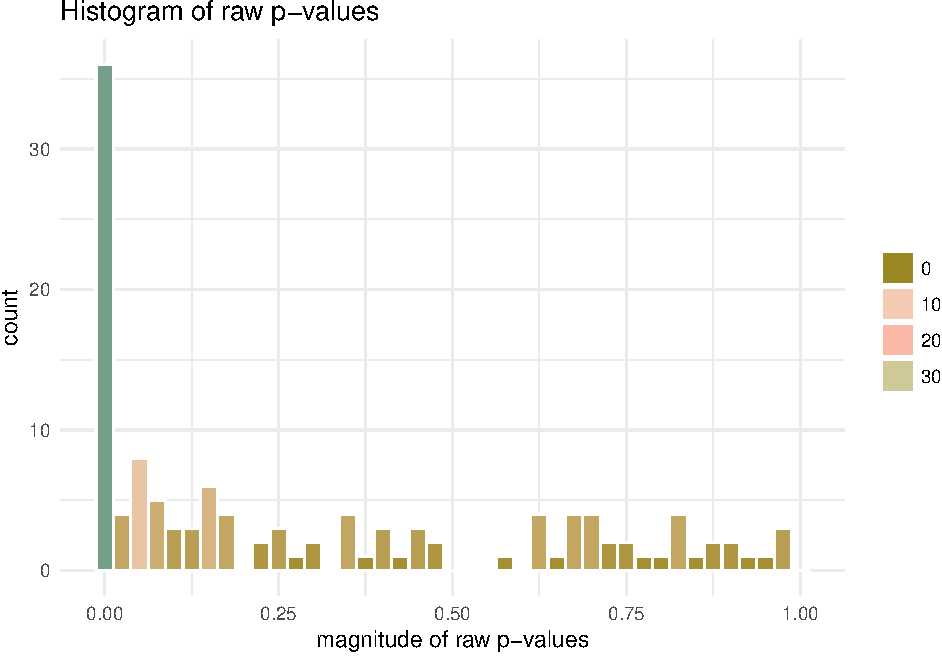
\includegraphics{paper_BiocF1000_files/figure-latex/methyvim-pvals-raw-1.pdf}

\begin{Shaded}
\begin{Highlighting}[]
\KeywordTok{plot}\NormalTok{(methyvim_cancer_ate, }\DataTypeTok{type =} \StringTok{"fdr_pvals"}\NormalTok{)}
\end{Highlighting}
\end{Shaded}

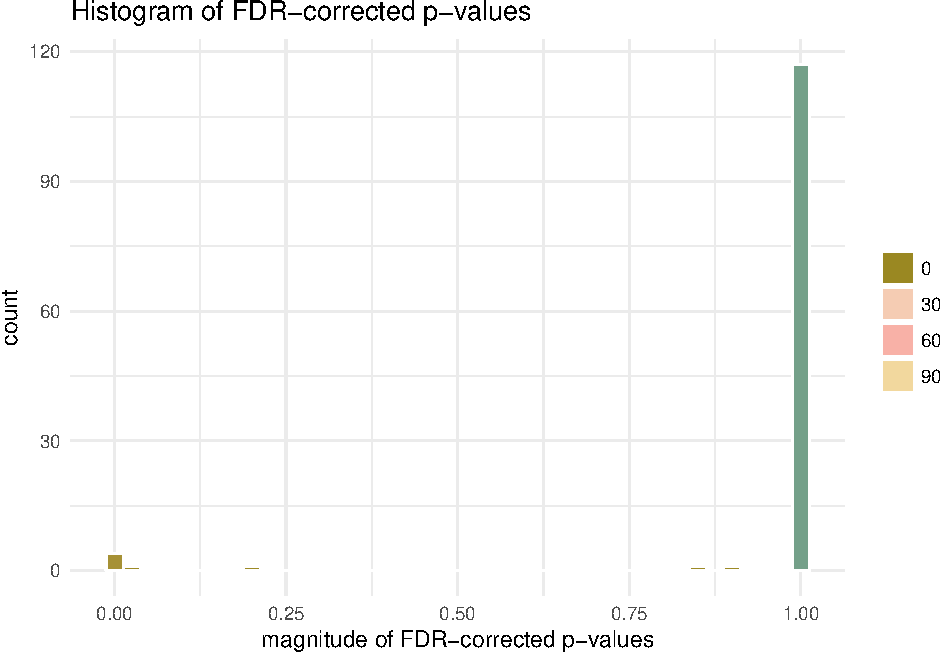
\includegraphics{paper_BiocF1000_files/figure-latex/methyvim-pvals-fdr-1.pdf}

\textbf{Remark:} The plots displayed above may also be generated as
side-by-side histograms in a single plot object. This is the default for
the \texttt{plot} method and may easily be invoked by specifying no
additional arguments to the \texttt{plot} function, unlike in the above.

While histograms of the p-values may be generally useful in inspecting
the results of the estimation procedure, a more common plot used in
examining the results of differential methylation procedures is the
volcano plot, which plots the parameter estimate along the x-axis and
\(-\text{log}_{10}(\text{p-value})\) along the y-axis. We implement such
a plot in the \texttt{methyvolc} function:

\begin{Shaded}
\begin{Highlighting}[]
\KeywordTok{methyvolc}\NormalTok{(methyvim_cancer_ate)}
\end{Highlighting}
\end{Shaded}

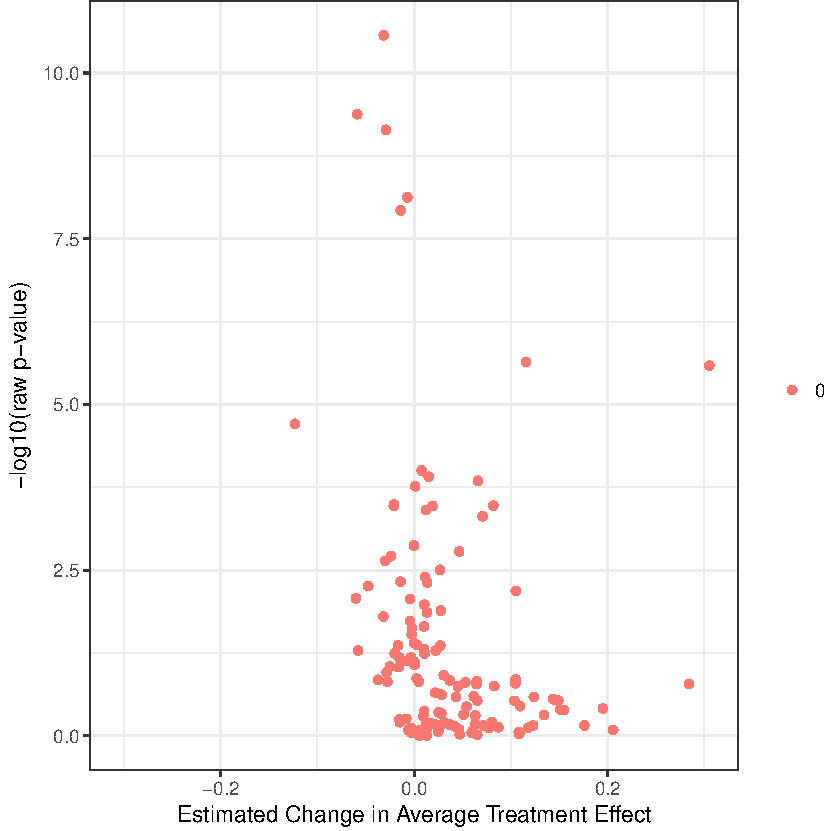
\includegraphics{paper_BiocF1000_files/figure-latex/methyvim-volcano-1.pdf}

The purpose of such a plot is to ensure that very low (possibly
statistically significant) p-values do not arise from cases of low
variance. This appears to be the case in the plot above (notice that
most parameter estimates are near zero, even in cases where the raw
p-values are quite low).

Yet another popular plot for visualizing effects in such settings is the
heatmap, which plots estimates of the raw methylation effects (as
measured by the assay) across subjects using a heat gradient. We
implement this in the \texttt{methyheat} function:

\begin{Shaded}
\begin{Highlighting}[]
\KeywordTok{methyheat}\NormalTok{(methyvim_cancer_ate)}
\end{Highlighting}
\end{Shaded}

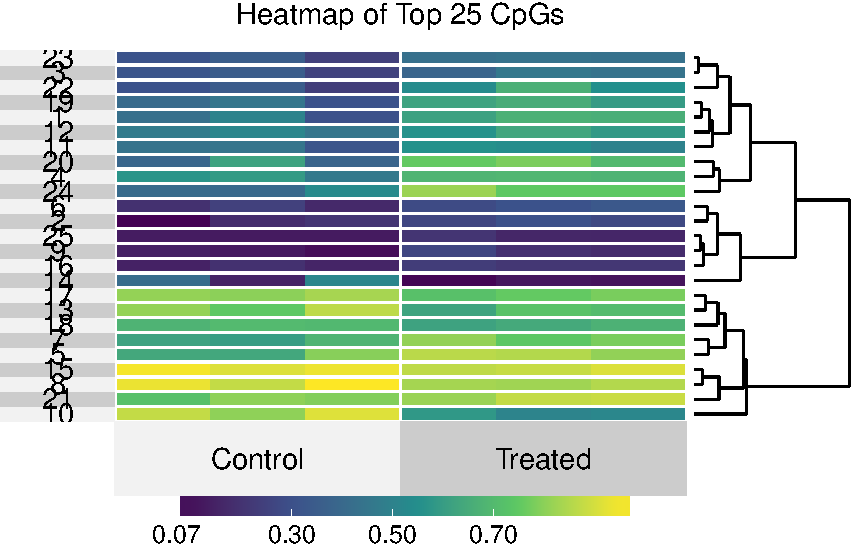
\includegraphics{paper_BiocF1000_files/figure-latex/methyvim-heatmap-1.pdf}

Invoking \texttt{methyheat} in this manner produces a plot of the top
sites (\(25\), by default) based on the raw p-value, using the raw
methylation measures in the plot. This uses the exceptional
\texttt{superheat} R package ({\textbf{???}}).

\section{Summary}\label{summary}

Here we introduce the R package \texttt{methyvim}, an algorithm for
differential methylation analysis that moves beyond linear models.
Additionally, this estimation procedure produces straightforward
statistical inference. Inspired by concepts of counterfactual effects
from the causal inference literature and machine learning algorithms, we
provide a computationally efficient technique for obtaining targeted
estimates of nonparametric variable importance measures for a
pre-screened set of CpGs, controlling for the False Discovery Rate as if
all sites were tested, and the estimation framework is built on targeted
minimum loss-based estimation. By taking advantage of the prediction
power of machine learning algorithms, this methodology targets the
individual importance of each CpG site, providing a fully nonparametric
statistical model for the analysis of differential methylation.

\section{Software availability}\label{software-availability}

Latest source code (development version):
\url{https://github.com/nhejazi/methyvim}

Bioconductor (stable release):
\url{https://bioconductor.org/packages/methyvim}

Archived source code as at time of publication:
\url{https://github.com/nhejazi/methyvim}

Software license: The MIT License, copyright Nima S. Hejazi

\section{Author contributions}\label{author-contributions}

NH designed and implemented the software package, applied the tool to
the use cases, and co-drafted the present article. RP helped in
designing the software and co-drafted the present article. AH and ML
serve as the advisors for the development of this software and general
statistical algorithm.

\section{Competing interests}\label{competing-interests}

No competing interests were disclosed.

\section{Grant information}\label{grant-information}

NH was supported in part by the National Library Of Medicine of the
National Institutes of Health under Award Number T32LM012417, by
{[}SUPERFUND GRANT{]}, and by {[}NINA HOLLAND GRANT{]}. RP was supported
by {[}SUPERFUND GRANT{]}. The content of this work is solely the
responsibility of the authors and does not necessarily represent the
official views of the various funding sources and agencies.

\section*{References}\label{references}
\addcontentsline{toc}{section}{References}

\hypertarget{refs}{}
\hypertarget{ref-benjamini1995controlling}{}
Benjamini, Yoav, and Yosef Hochberg. 1995. ``Controlling the False
Discovery Rate: A Practical and Powerful Approach to Multiple Testing.''
\emph{Journal of the Royal Statistical Society. Series B
(Methodological)}. JSTOR, 289--300.

\hypertarget{ref-chambaz2012estimation}{}
Chambaz, Antoine, Pierre Neuvial, and Mark J van der Laan. 2012.
``Estimation of a Non-Parametric Variable Importance Measure of a
Continuous Exposure.'' \emph{Electronic Journal of Statistics} 6. NIH
Public Access: 1059.

\hypertarget{ref-hernan2018causal}{}
Hernan, Miguel A, and James M Robins. 2018, forthcoming. \emph{Causal
Inference}. Chapman \& Hall/Crc Texts in Statistical Science. Taylor \&
Francis.

\hypertarget{ref-libbrecht2015machine}{}
Libbrecht, Maxwell W, and William Stafford Noble. 2015. ``Machine
Learning in Genetics and Genomics.'' \emph{Nature Reviews. Genetics} 16
(6). NIH Public Access: 321.

\hypertarget{ref-pearl2009causality}{}
Pearl, Judea. 2009. \emph{Causality: Models, Reasoning, and Inference}.
Cambridge University Press.

\hypertarget{ref-robertson2005dna}{}
Robertson, Keith D. 2005. ``DNA Methylation and Human Disease.''
\emph{Nature Reviews. Genetics} 6 (8). Nature Publishing Group: 597.

\hypertarget{ref-tuglus2008targeted}{}
Tuglus, Catherine, and Mark J van der Laan. 2008. ``Targeted Methods for
Biomarker Discovery, the Search for a Standard.'' bepress.

\hypertarget{ref-tuglus2009modified}{}
Tuglus, Catherine, and Mark J. van der Laan. 2009. ``Modified FDR
Controlling Procedure for Multi-Stage Analyses.'' \emph{Statistical
Applications in Genetics and Molecular Biology} 8 (1). Walter de
Gruyter: 1--15.
doi:\href{https://doi.org/10.2202/1544-6115.1397}{10.2202/1544-6115.1397}.

\hypertarget{ref-vdl2006statistical}{}
van der Laan, Mark J. 2006. ``Statistical Inference for Variable
Importance.'' \emph{The International Journal of Biostatistics} 2 (1).

\hypertarget{ref-vdl2011targeted}{}
van der Laan, Mark J, and Sherri Rose. 2011. \emph{Targeted Learning:
Causal Inference for Observational and Experimental Data}. Springer
Science \& Business Media.

\hypertarget{ref-vdl2017targeted}{}
---------. 2017. \emph{Targeted Learning in Data Science: Causal
Inference for Complex Longitudinal Studies}. Springer Science \&
Business Media.

\hypertarget{ref-vdl2006targeted}{}
van der Laan, Mark J, and Daniel Rubin. 2006. ``Targeted Maximum
Likelihood Learning.'' \emph{The International Journal of Biostatistics}
2 (1).

\end{document}
